%\vspace*{-3mm}
\pstart\noindent
\lbrack80~v\textsuperscript{o}\rbrack\ \setline{1}
\pend
\vspace{0.5em}
\pstart
\centering
%\vspace*{-5mm}
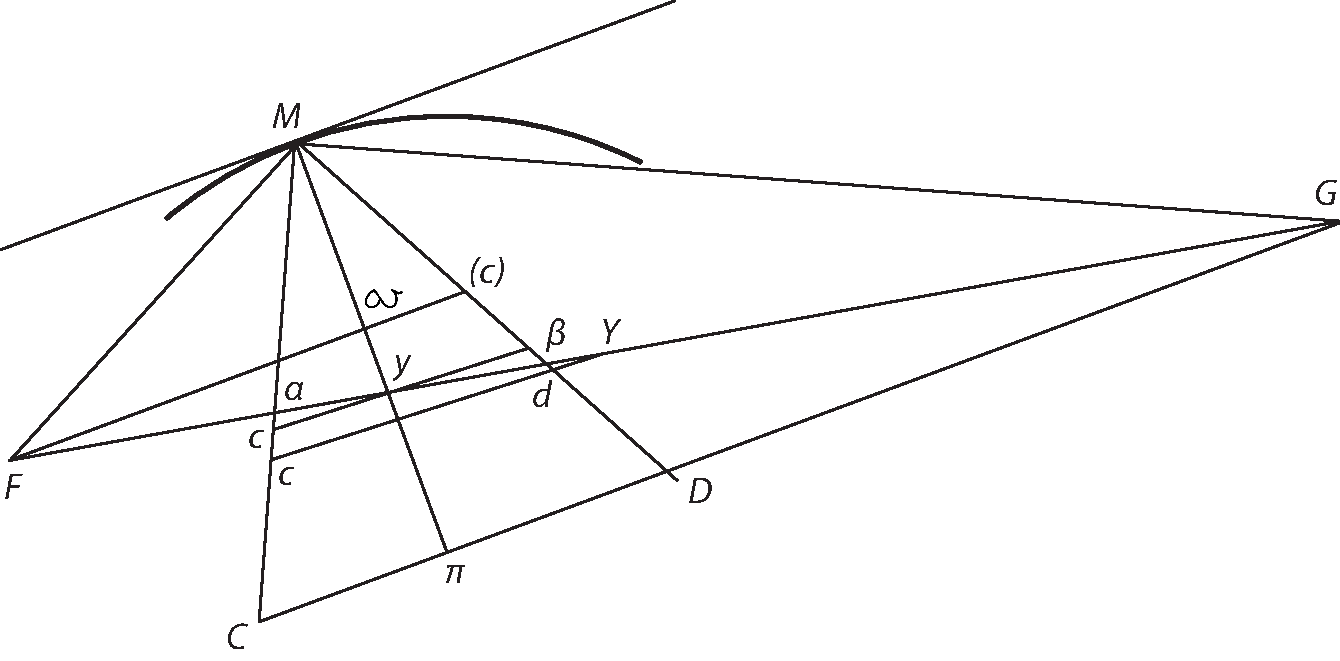
\includegraphics[width=1\textwidth]{images/LH037,03_080v-d1.pdf}\\
\centering[\textit{Fig. 4}]
\pend
\newpage
\pstart
$F$ $G$ puncta fixa. $M$ punctum curvae quodcunque. Angulus $FMD$ rectus. \edtext{[Angulus]}{\lemma{}\Bfootnote{Angulus \textit{\ erg. Hrsg.}}} $GMC$ \edtext{[rectus]}{\lemma{}\Bfootnote{rectus \textit{\ erg. Hrsg.}}}. Recta $GDC$ parallela, rectae $M$ tangenti. 
\rule[-4mm]{0mm}{10mm}$\displaystyle\frac{FMD}{GMC}$ sit ratio data constans quaeritur natura curvae. Majoris aequitatis causa rectam tangenti parallelam ducamus neque per $F$ neque per $G,$ sed per $Y$ punctum medium inter $F$ $G$ ut utrumque punctum fixum eodem modo tractetur vel si geometricum ut ita dicam aequitatem obtinere velimus ducemus parallelam non per $\alpha$ vel $\beta$ sed per $y$ ponendo esse $\alpha y$ ad $\beta y$ ut $F\alpha$ ad $G\beta$. Nihil autem ad summam rerum refert quaenam ex tot diversis $C$ $D$ eligamus. Sed satius erit ea, quae respondeat ipsi $y$. Sumi ita enim Triangula similia varia commodius communi scilicet. 
\pend
\pstart
Sed quaeritur quomodo curvae quaesitae naturam inveniamus.
\pend
\count\Afootins=1200
\count\Bfootins=1200
\count\Cfootins=1200
\pstart
Debet esse
\rule[-4mm]{0mm}{10mm}$\displaystyle\frac{FM}{GM}{\smallfrown\atop}\frac{MD}{MC}\, \sqcap$\textsuperscript{datur} $\displaystyle\frac{a}{b}.$
\pend
%\vspace{1mm}
\pstart
Sit \rule[-4mm]{0mm}{10mm}$a\sqcap b$ fiet $\displaystyle\frac{MD}{MC}\sqcap\frac{GM}{FM}$
\pend
%\vspace{1mm}
\pstart
Ad tangentem curvae ducatur perpendicularis $M\dsig\pi$. Habebimus Triangula \edtext{similia duo: $(C)F:FM:M(C)::MF:F\dsig:\dsig M::(C)M:\dsig M:\dsig(C)$ item $CG:GM:MC::MG:G \pi : \pi M::CM:M \pi : \pi C$.%
}{\lemma{similia}\Bfootnote{%
\textit{(1)}\ aliquot\ %
\textit{(2)}\ duo:\ %
\textit{(a)}\ $MF:F\dsig:(\dsig M):$\ %
\textit{(b)}\ $MF:(F\dsig ): \dsig M::MC. \dsig M: \dsig C$ item $MG$\ %
\textit{(c)}\ $(C)F:FM:M(C)$ [...] $CM:M \pi : \pi C$.\ \textit{L}}}
\pend
\pstart
Quaeritur $M\dsig$ vel $M\pi.$
\pend
\pstart\rule[-4mm]{0mm}{10mm}
$\overline{\dsig M}^2\sqcap F\dsig, \dsig C$ \quad
$\displaystyle\frac{\dsig M}{MF}\sqcap\frac{\dsig C}{CM}$ \quad
$\displaystyle\dsig M\sqcap\frac{\dsig C,MF}{CM}\sqcap\sqrt{F\dsig,\dsig C}$
\pend
\pstart
Ergo \rule[-4mm]{0mm}{10mm}$\displaystyle\frac{\dsig^2,MF^2}{CM^2}\sqcap F\dsig,\dsig C,$ et $\displaystyle\dsig C\sqcap\frac{F\dsig,CM^2}{MF^2}$ et $\displaystyle\dsig M\sqcap\frac{F\dsig,\overline{CM}^2}{MF^2},\frac{MF}{CM}\sqcap\frac{F\dsig,CM}{MF}.$
\pend
\pstart
Ergo \rule[-4mm]{0mm}{10mm}$\displaystyle\dsig M\sqcap\frac{F\dsig,CM}{MF},$ sed $F\dsig\sqcap\sqrt{\overline{FM}^2-\dsig M^2}$ fiet $\displaystyle\dsig M\sqcap\sqrt{FM^2-\dsig M^2},\frac{CM}{CF},$ seu $\displaystyle\frac{\dsig M^2,MF^2}{CM^2}\sqcap FM^2-\dsig M^2$ seu $\dsig M^2,MF^2,\sqcap FM^2,CM^2-\dsig M^2,CM^2$ seu $\displaystyle\dsig M\sqcap\frac{FM^2,CM^2}{MF^2+CM^2},$ seu \rule[-4mm]{0mm}{10mm}$\displaystyle\frac{MF^2+CM^2}{FM^2,CM^2}\sqcap\frac{1}{\dsig M^2}$ seu $\displaystyle\frac{1}{CM^2}+\frac{1}{MF^2}\sqcap\frac{1}{\dsig M^2}$
\pend
\newpage
\pstart
Alia curva talis, ut ad eam semper vectis\protect\index{Sachverzeichnis}{vectis} ducens eundem faciat angulum, exempli causa, ut semper eam tangat, ita frictio\protect\index{Sachverzeichnis}{frictio} perpetua eadem, ut non minuitur, sed fit potius 
\edtext{major; quia}{\lemma{major;}\Bfootnote{\textit{(1)}\ et \textit{(2)}\ quia \textit{L}}} 
perpetuo tota portio 
\edtext{curvae vecti\protect\index{Sachverzeichnis}{vectis}}{\lemma{curvae}\Bfootnote{\textit{(1)}\ rectae \textit{(2)}\ vecti \textit{L}}} 
\edtext{affricatur.\\%
\indent%
Minima}{\lemma{affricatur}\Bfootnote{%
\textit{(1)} at praeterea %
\textit{(2)}~. Minima \textit{L}}}
frictio\protect\index{Sachverzeichnis}{frictio} erit si, vectis\protect\index{Sachverzeichnis}{vectis} ducens semper sit ad curvam perpendicularis. Sed tunc cum circulus ex vectis\protect\index{Sachverzeichnis}{vectis} centro longitudine vectis\protect\index{Sachverzeichnis}{vectis} descriptus curvam tangat, utique non ducet. 
\pend
\vspace{1em}
\pstart
%\begin{wrapfigure}[5]{l}{0.12\textwidth}
\centering
\vspace{1em}
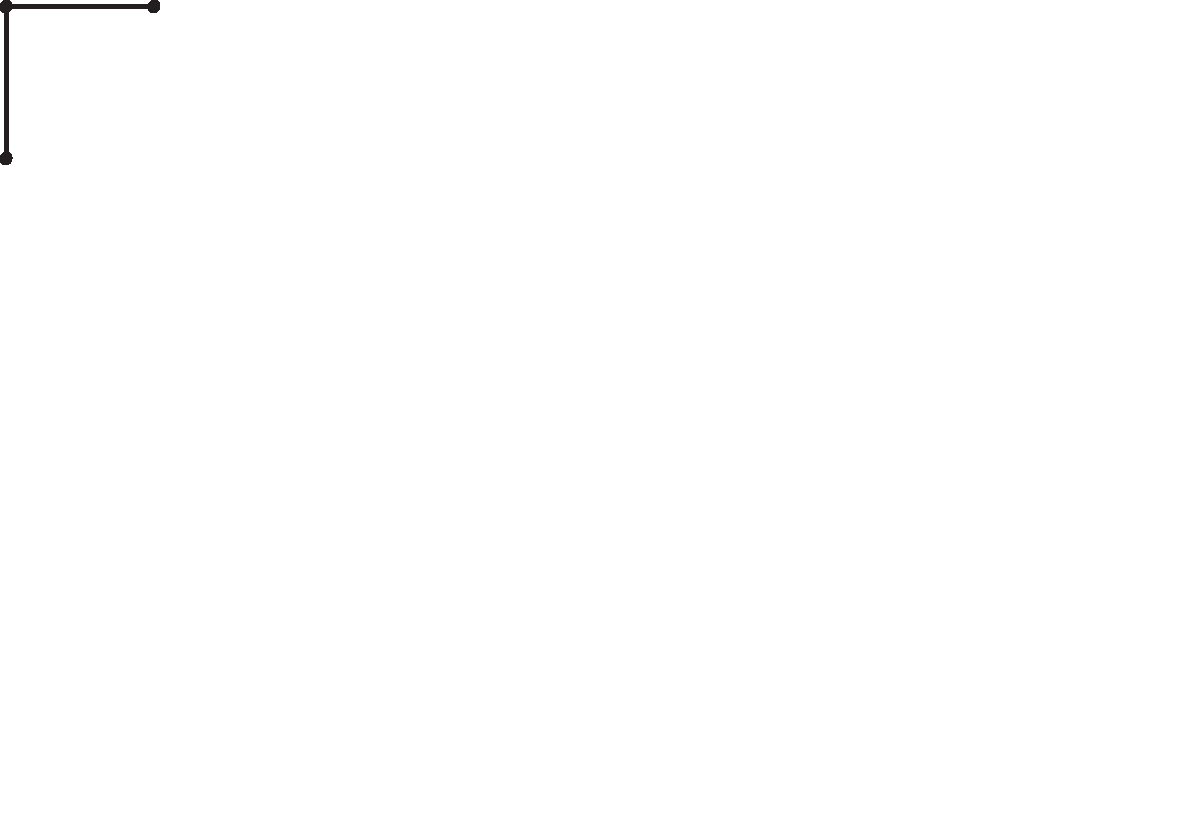
\includegraphics[trim = 0mm -3mm 0mm 0mm, clip, width=0.12\textwidth]{images/LH037,03_080v-d2.pdf}\\
\noindent \centering [\textit{Fig. 5}]
\pend
\vspace{1em}
\pstart
Medium\setline{7} ita eligemus, si vectis\protect\index{Sachverzeichnis}{vectis}  
\edtext{ducens semper ad tangentem curvae faciat}{\lemma{ducens}\Bfootnote{ \textit{(1)}\ sit \textit{(2)}\  semper [...] faciat \textit{ L}}} angulum 45\setline{11} graduum.
\pend
\vspace{1.5em}
\pstart
\centering 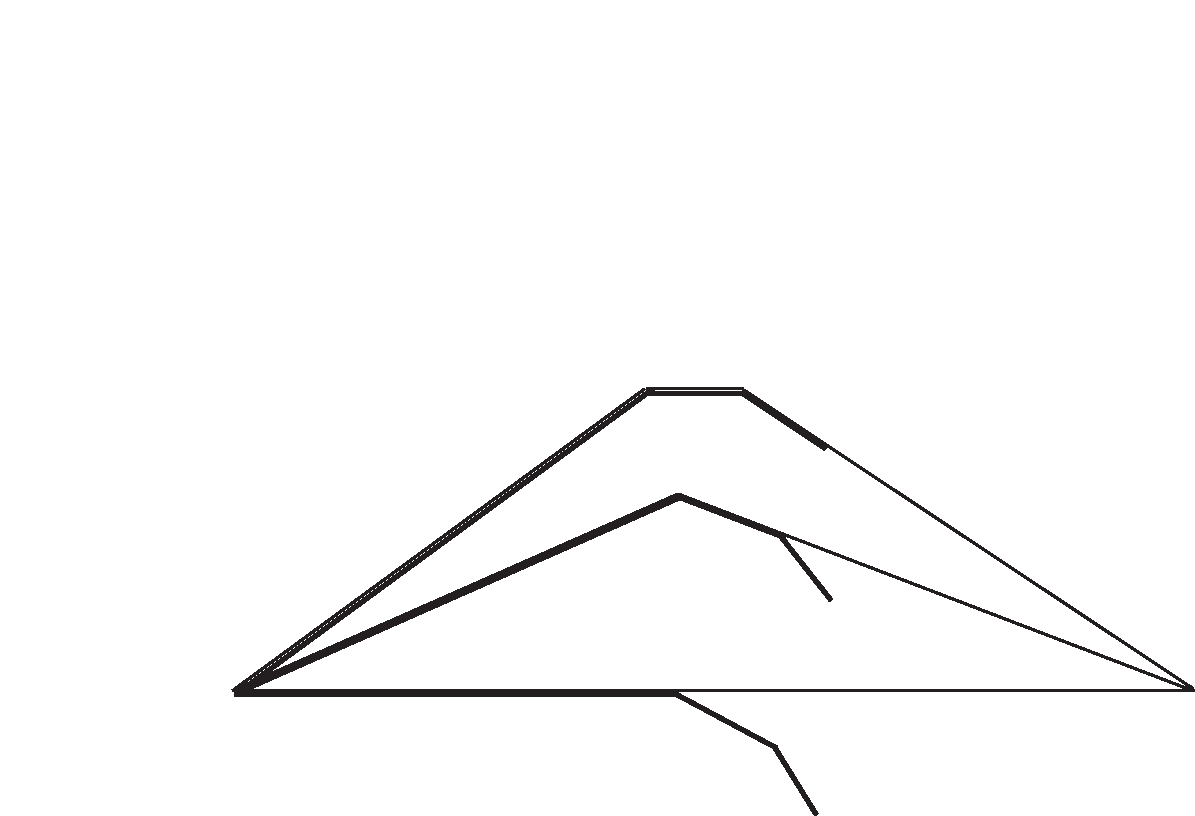
\includegraphics[trim = 0mm -3mm 0mm 0mm, clip, width=0.45\textwidth]{images/LH037,03_080v-d3.pdf}\\
\centering [\textit{Fig. 6}]
\pend
\count\Afootins=1500
\count\Bfootins=1500
\count\Cfootins=1500

